\subsection{Low-\texorpdfstring{$\ell$}{ℓ} CMB Power Suppression from Global Projective Coherence Constraints}
  \label{app:lowell_attenuation}

  The lowest CMB multipoles probe global properties of
  $\chi_{\mathrm{eff}}$ rather than independent local perturbations
  (Sections~\ref{subsec:cmb},~\ref{subsec:large-angle-anomalies}).
  Because the finite projective capacity of~$\chi$ limits how globally
  coherent configurations can deviate from the admissible background, the
  lowest $\ell$-modes are systematically attenuated.

  \begin{figure}[htbp]
    \centering
    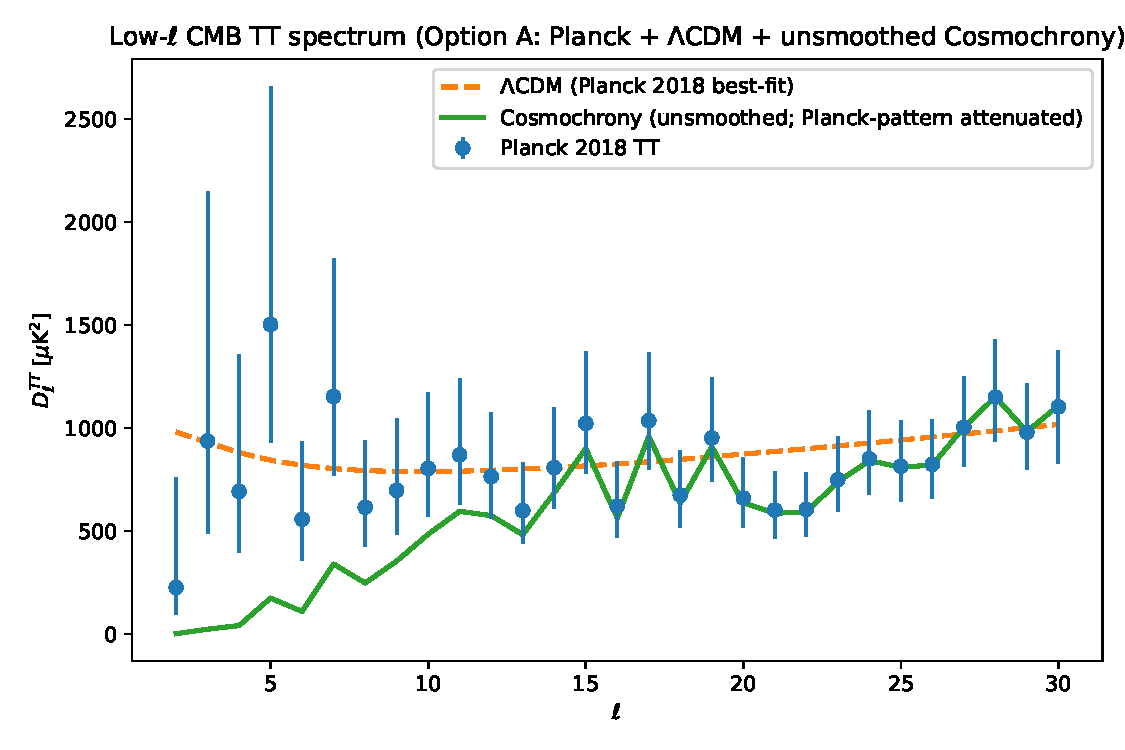
\includegraphics[width=0.85\textwidth]
    {6-appendices/appC/001-cmb_lowell_unsmoothed}
    \caption{Observed CMB temperature power spectrum at low multipoles.
    The shaded region illustrates a qualitative attenuation envelope
    from global projective coherence constraints.}
    \label{fig:cmb_lowell_unsmoothed}
  \end{figure}

  \paragraph{Significance of the unsmoothed comparison.}
    Figure~\ref{fig:cmb_lowell_unsmoothed} is not intended as a precision fit,
    but as a structural diagnostic.
    Unlike a sharp infrared cutoff or a purely statistical suppression,
    the attenuation mechanism preserves the relative multipole-to-multipole
    variations observed in the Planck data.
    As $\ell \rightarrow 0$, the same increasing and decreasing trends are
    reproduced, albeit with a progressively reduced amplitude.

    This behavior is non-trivial.
    In $\Lambda$CDM, the lowest multipoles are treated as cosmic-variance–dominated
    outliers, with no underlying mechanism constraining their relative structure.
    Here, the correlated attenuation emerges from a single global constraint:
    the finite projective coherence capacity of $\chi_{\mathrm{eff}}$.

  \paragraph{Distinguishable-history mechanism.}
    The quantitative carrier of this constraint is now identified~\cite{Beau2026dhc}.
    At the largest angular scales, the relevant modes probe the first admissibility ranks of the
    projective description.
    The suppression mechanism is therefore not an adjustable dynamical damping term: it follows
    from the small absolute number of distinguishable projective histories available at those
    ranks.
    In the canonical counting channel~\cite{Beau2026tb} this number is
    \[
      N_{\mathrm{hist}}(n)
      = \frac{(1+\sqrt{2})^{n+1}+(1-\sqrt{2})^{n+1}}{2},
    \]
    so the first ranks contain only $3$, $7$, and $17$ distinguishable histories, and the
    large-angle deficit is a small-$N$ distinguishable-history effect.
    The comparison with CMB data must be made by applying the derived history envelope to the
    $\Lambda$CDM spectrum, not by attenuating the observed Planck points; the resulting no-fit,
    quadrupole-anchored envelopes improve the Planck TT low-$\ell$ diagnostic without any adjusted
    parameter~\cite{Beau2026dhc}.

  \paragraph{Phenomenological parametrization (descriptive diagnostic only).}
    The envelope
    \begin{equation}
      C_\ell^{\mathrm{CC}}
      = C_\ell^{\Lambda\mathrm{CDM}}
      \left[
        1 - \alpha
        \exp\!\left(-\frac{\ell}{\ell_0}\right)
      \right],
      \quad
      \alpha \in [0,1],\;\ell_0 > 0,
      \label{eq:cc_lowell_envelope}
    \end{equation}
    used in earlier versions of this appendix has two free parameters and is retained only as a
    descriptive diagnostic; it is superseded as the core claim by the parameter-free count-derived
    envelope of~\cite{Beau2026dhc}.

  \paragraph{Graph-theoretic admissibility filter.}
    The weighted Laplacian $L_G(t)$ of the relational connectivity graph
    sets a minimal nonzero eigenvalue $\lambda_2(t)$ characterizing global
    connectivity.
    The primordial power spectrum is modulated by
    \[
      \mathcal{A}(k,t)
      = \exp\!\left[
                -\left(
                   \frac{\lambda_2(t)}{k^2}
        \right)^{\!p/2}
      \right],
    \]
    reflecting the inability of an insufficiently connected relational graph
    to support large-scale coherent modes.
